\subsection{Sous-mission A3}

	\begin{vwcol}[widths={0.65,0.2}, rule=0pt]
	\begin{minipage}{0.7\textwidth}
	\paragraph{Objectifs de la mission}

	Mettre en valeur les caneaux d'eau chaude sur une image en nuances de gris
	\end{minipage}

	\begin{minipage}{0.25\textwidth}
	\begin{flushright}
	\paragraph{Technique utilisée}
	
	Seuillage\up{\ref{Seuillage}}
	\end{flushright}
	\end{minipage}

	\end{vwcol} 

	\begin{figure}[h]
	\centering
		\begin{multicols}{2}
		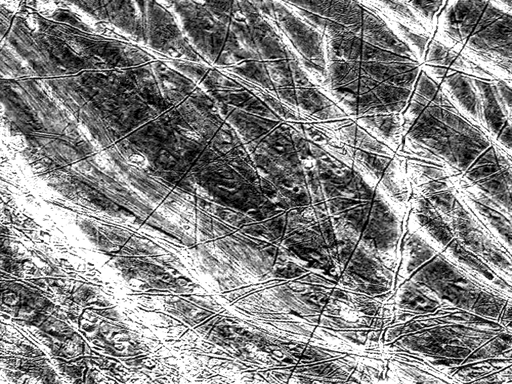
\includegraphics[scale=0.5]{images/Europa_surface.png}
		Avant

		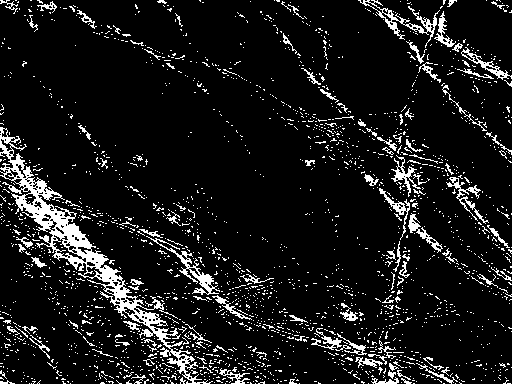
\includegraphics[scale=0.5]{images/MissionA3.png}
		Après
		\end{multicols}
	\end{figure}
	\vspace{-0.9cm}

	\paragraph{Procédé}	
		L'objectif de cette mission était de cartographier la circulation de l'eau sous la surface glacée de l'astre en ne faisant apparaître que les canaux d'eau chaude. Pour remplir la mission, nous avons utilisés un \emph{seuillage}. Afin d'observer les zones chaudes qui apparaissent en blanc.